\section{Introduction}
\label{sec:introduction}

Instructional Systems Design (ISD) is a systematic process for creating effective learning experiences, encompassing five phases: Analysis, Design, Development, Implementation, and Evaluation, commonly known as the ADDIE model~\cite{branson1975addie}. ISD determines the quality and effectiveness of educational programs across diverse contexts, from corporate training to academic curricula. However, ISD is inherently a complex, multi-step task that requires human experts to execute each phase carefully. The process demands collaboration among instructional designers, subject matter experts, and multimedia specialists, with project timelines typically spanning weeks to months depending on scope and complexity. This significant investment of time and resources limits the scalability of high-quality ISD.

Recent advances in Large Language Models (LLMs) have sparked interest in applying them to ISD tasks. Hu et al.~\cite{hu2024teachingplan} explored GPT-4's potential for teaching plan generation and evaluation, while LessonPlanner~\cite{lessonplanner2024} assists novice teachers in preparing pedagogy-driven lesson plans. However, these approaches remain at the level of \textit{assisting} human designers rather than automating the full ISD process. The core design decisions and iterative refinements still require human expertise.

\begin{figure*}[t]
\centering
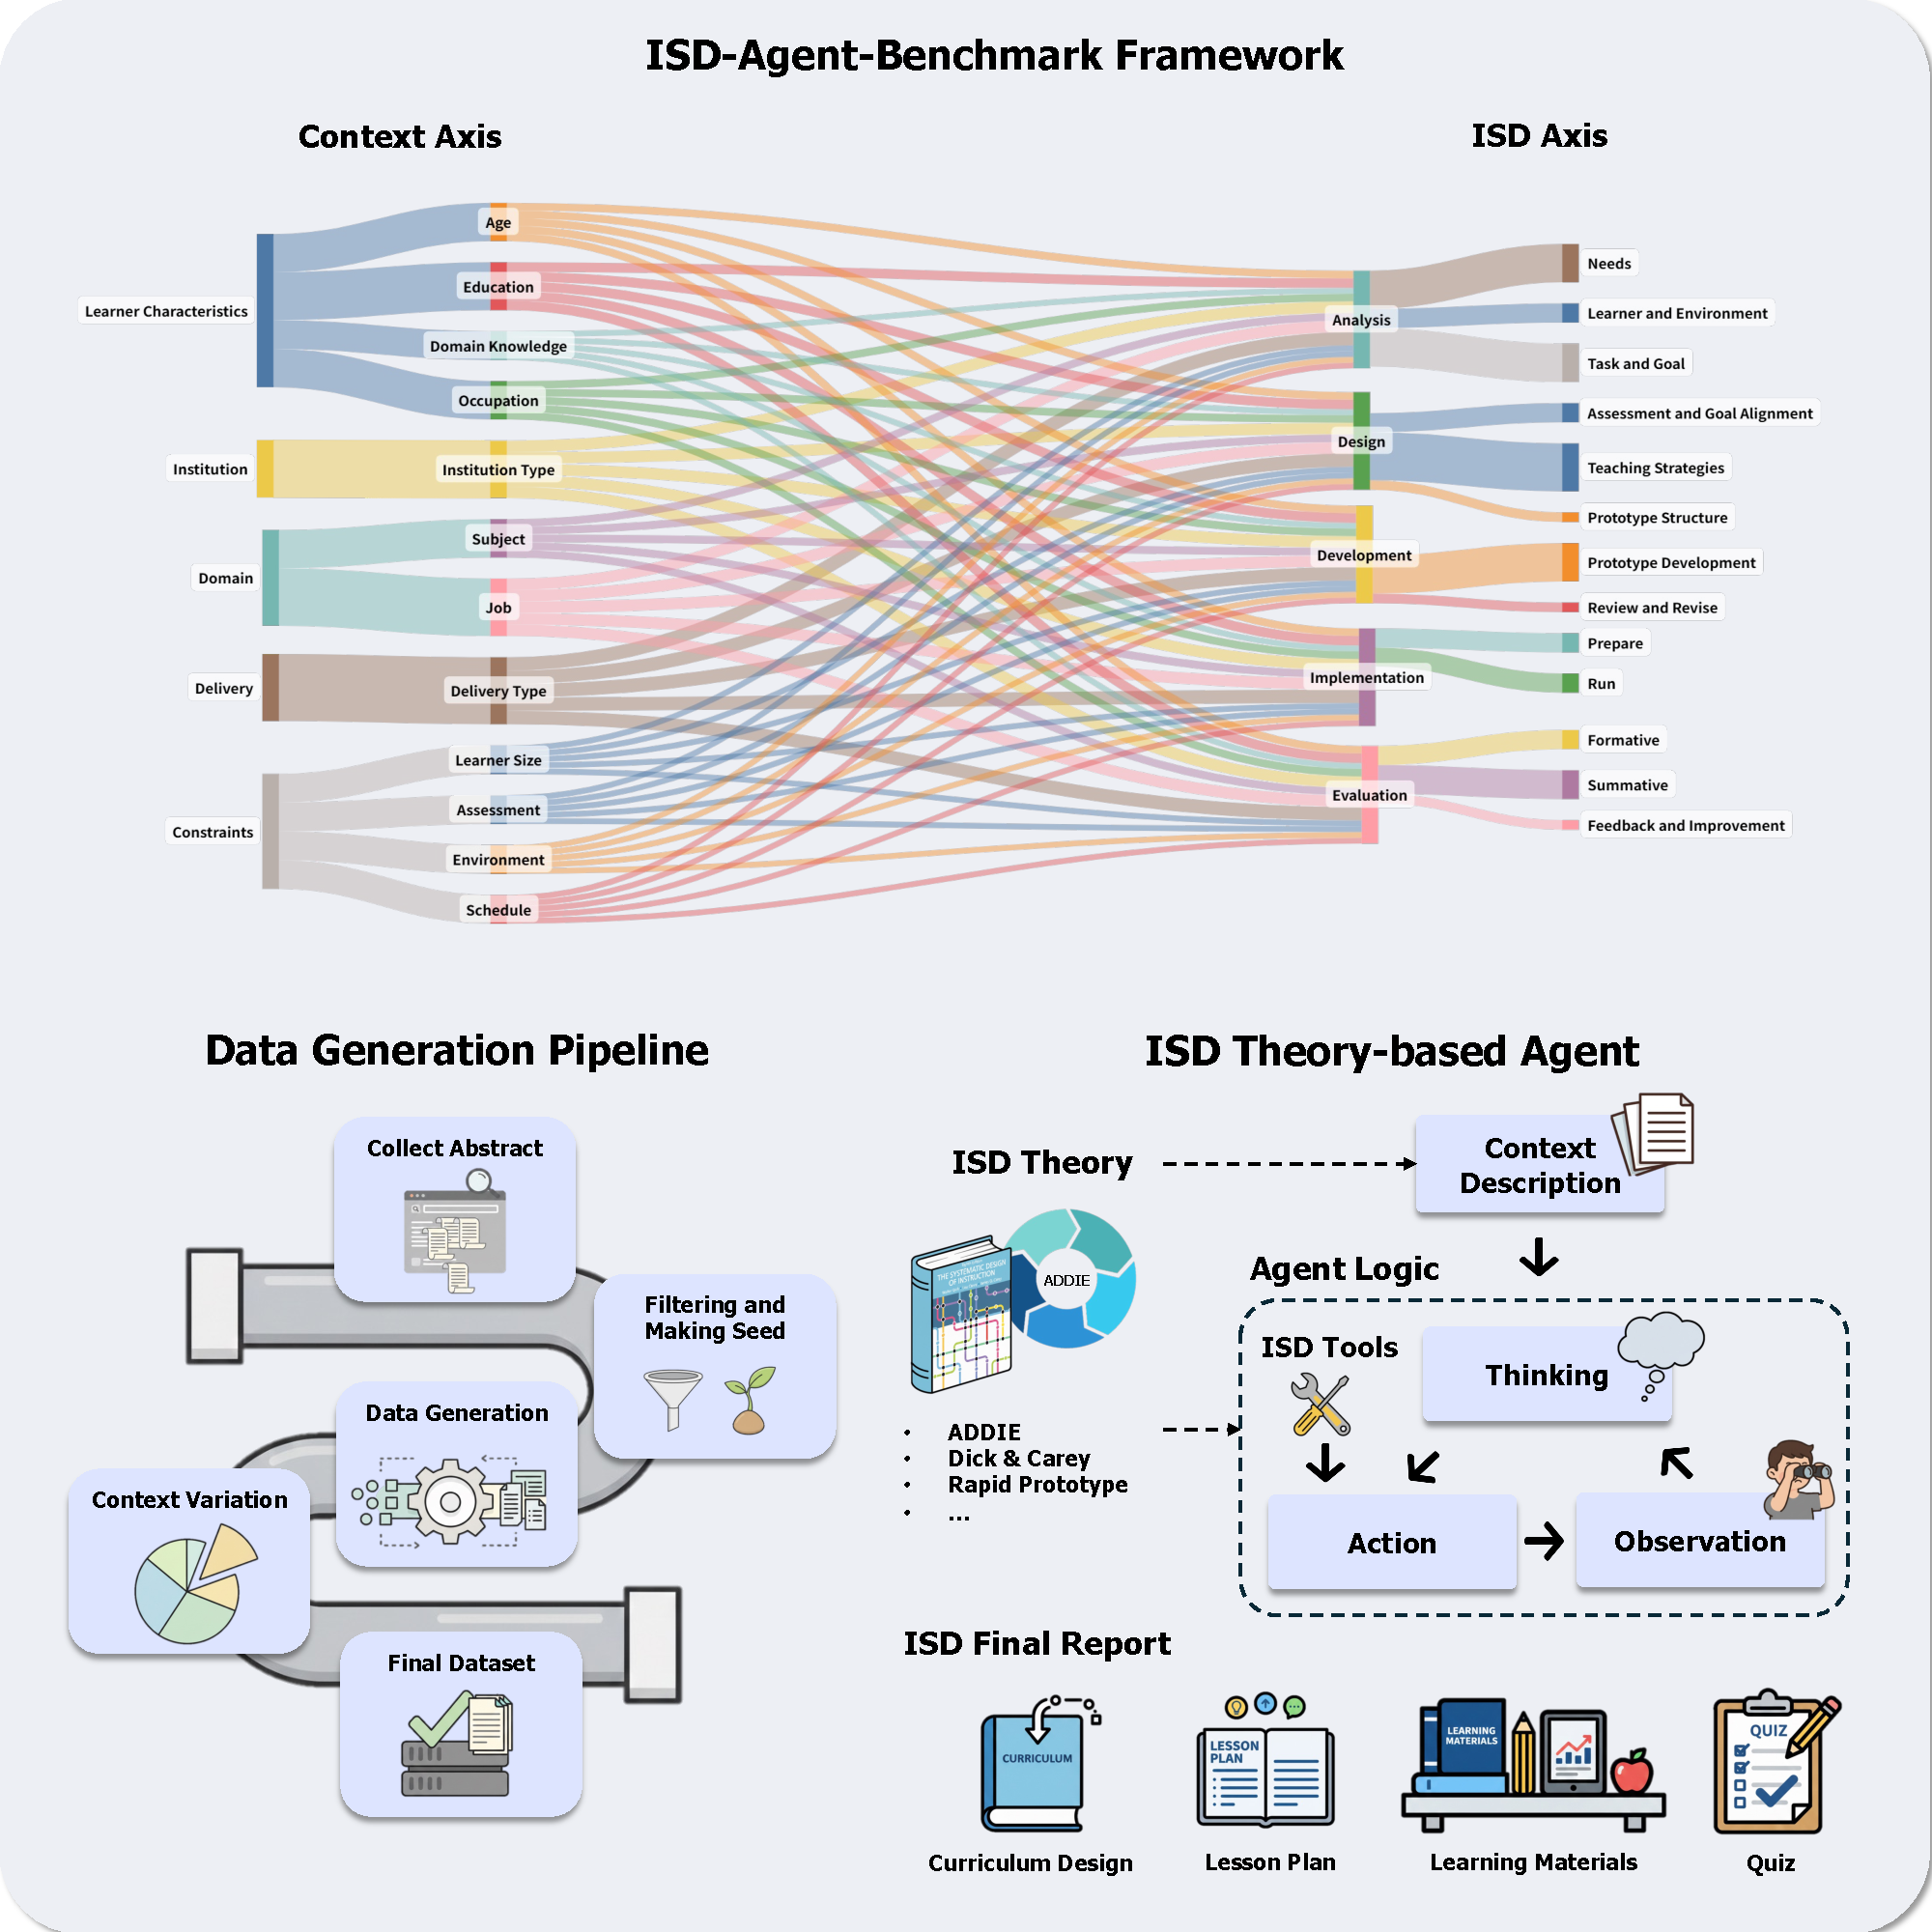
\includegraphics[width=0.8\textwidth]{main_figure_v8.pdf}
\caption{Overview of ISD-Agent-Bench. \textit{Top} is the Context Matrix framework that combines 51 contextual variables across 5 categories (Learner Characteristics, Institution, Domain, Delivery, Constraints) with the ISD Matrix containing 33 ADDIE-based sub-steps for systematic scenario generation. \textit{Bottom left} is the data generation pipeline from abstract collection through context variation to final dataset. \textit{Bottom right} is the ISD theory-based agent architecture integrating classical ISD theories with ReAct-style reasoning to produce comprehensive ISD outputs.}
\label{fig:teaser}
\end{figure*}

Meanwhile, LLM-based agents, systems that use LLMs as central controllers to perceive environments, formulate plans, utilize tools, and execute tasks autonomously~\cite{wang2024llmagentsurvey}, have advanced rapidly across diverse domains. In software engineering, agents now resolve real-world GitHub issues~\cite{jimenez2024swebench}; in web navigation, they complete complex multi-step tasks autonomously~\cite{zhou2023webarena}. The evaluation of such agents has also matured, with benchmarks like AgentBench~\cite{liu2023agentbench} assessing capabilities across interactive environments. Notably, agent benchmarks are fundamentally more challenging to develop than traditional LLM benchmarks: while LLMs are evaluated on text generation or question answering, agents operate in dynamic, interactive environments requiring reasoning, planning, tool use, and real-world effects~\cite{mohammadi2025agenteval}.

Despite these advances, research on LLM agents for instructional systems design remains scarce. EduPlanner~\cite{zhang2025eduplanner} applies multi-agent systems to mathematics lesson design, and Instructional Agents~\cite{yao2025instructionalagents} automates course material generation. However, no comprehensive benchmark exists for systematically evaluating ISD agents. Existing educational benchmarks such as EduBench~\cite{edubench2025} and TutorBench~\cite{tutorbench2025} focus on direct LLM evaluation for tutoring or content knowledge, rather than agentic systems addressing the full ISD lifecycle.

To address this gap, we present \benchmark{}\footnote{\url{https://anonymous.4open.science/r/isd-agent-benchmark-8D77}}, the first comprehensive benchmark for evaluating LLM-based ISD agents (Figure~\ref{fig:teaser}). Our benchmark introduces a Context Matrix framework that systematically combines 51 contextual variables with 33 ISD sub-steps derived from the ADDIE model, generating \numscenarios{} diverse scenarios with \numtest{} test cases. The evaluation methodology combines ADDIE-based rubric assessment with trajectory analysis, enabling holistic evaluation of both output quality and agent behavior.

Furthermore, we propose four ISD theory-based agents: React-ADDIE, which integrates the ADDIE framework with ReAct-style reasoning; ADDIE-Agent with fine-grained phase decomposition; Dick-Carey-Agent based on Dick \& Carey's systematic design~\cite{dick1978systematic}; and RPISD-Agent based on Rapid Prototyping ISD~\cite{tripp1990rapid}. Evaluating across three LLMs (Gemini-3-Flash, GPT-5-mini, Solar-Pro3) with a multi-judge protocol achieving 0.905 reliability, our experiments reveal that React-ADDIE achieves the highest performance (86.49 points), demonstrating that the synergy between classical ISD theory and modern agent architectures produces superior outcomes compared to either pure theory-based approaches (ADDIE-Agent: 82.96) or technique-only baselines (84.07).

\subsection{Contributions}
\label{subsec:contributions}

Our contributions are fourfold:

\begin{itemize}
    \item \textbf{Context Matrix Framework}: We propose a two-dimensional framework combining 51 contextual variables across 5 categories with 33 ISD sub-steps for systematic scenario generation, enabling comprehensive coverage of the ISD space.

    \item \textbf{Large-scale Benchmark}: We construct \benchmark{} with \numscenarios{} scenarios and \numtest{} test cases, featuring stratified sampling across 9 contextual dimensions including learner characteristics, institutional context, and difficulty levels.

    \item \textbf{ISD Theory-based Agents}: We develop four agents grounded in classical ISD theories (React-ADDIE, ADDIE-Agent, Dick-Carey-Agent, RPISD-Agent), demonstrating that integrating traditional ISD frameworks with modern agent architectures yields superior performance.

    \item \textbf{Comprehensive Analysis}: We conduct extensive experiments revealing that ISD theory functions as quality assurance rather than performance optimization, with theory value amplifying as task complexity increases.
\end{itemize}
